%%%%%%%%%%%%%%%%%%%%%%%%%%%%% Define Article %%%%%%%%%%%%%%%%%%%%%%%%%%%%%%%%%%
\documentclass{beamer}
\usetheme{CambridgeUS}
%%%%%%%%%%%%%%%%%%%%%%%%%%%%%%%%%%%%%%%%%%%%%%%%%%%%%%%%%%%%%%%%%%%%%%%%%%%%%%%

%%%%%%%%%%%%%%%%%%%%%%%%%%%%% Using Packages %%%%%%%%%%%%%%%%%%%%%%%%%%%%%%%%%%
\usepackage{graphics}
\usepackage{booktabs}
\usepackage{siunitx}
\usepackage{amsmath}
\usepackage{inputenc}


%%%%%%%%%%%%%%%%%%%%%%%%%%%%% Other settings %%%%%%%%%%%%%%%%%%%%%%%%%%%%%%%%%%
\sisetup{input-symbols = {()},  % do not treat "(" and ")" in any special way
         group-digits  = false} % no grouping of digits
\DeclareUnicodeCharacter{200D}{-}
%%%%%%%%%%%%%%%%%%%%%%%%%%%%%%%%%%%%%%%%%%%%%%%%%%%%%%%%%%%%%%%%%%%%%%%%%%%%%%%

%%%%%%%%%%%%%%%%%%%%%%%%%%%%%%% Title & Author %%%%%%%%%%%%%%%%%%%%%%%%%%%%%%%%
\title[Under- Over-Reaction in TSE]{Do We Have Under- Over-Reaction in TSE?}
\subtitle[]{Supervised by: Dr.\ Mahdi Heidari}
\author[Heidari, Mir]{Mahdi Mir}
\institute[]{TeIAS}
%%%%%%%%%%%%%%%%%%%%%%%%%%%%%%%%%%%%%%%%%%%%%%%%%%%%%%%%%%%%%%%%%%%%%%%%%%%%%%%

%%%%%%%%%%%%%%%%%%%%%%%%%%%%%%% Document Start %%%%%%%%%%%%%%%%%%%%%%%%%%%%%%%%
\begin{document}
%%%%%%%%%%%%%%%%%%%%%%%%%%%%%%%%%%%%%%%%%%%%%%%%%%%%%%%%%%%%%%%%%%%%%%%%%%%%%%%

%%%%%%%%%%%%%%%%%%%%%%%%%%%%%%%%%%%%%%%%%%%%%%%%%%%%%%%%%%%%%%%%%%%%%%%%%%%%%%%
\maketitle
%%%%%%%%%%%%%%%%%%%%%%%%%%%%%%%%%%%%%%%%%%%%%%%%%%%%%%%%%%%%%%%%%%%%%%%%%%%%%%%

%%%%%%%%%%%%%%%%%%%%%%%%%%%%%%%%%%%%%%%%%%%%%%%%%%%%%%%%%%%%%%%%%%%%%%%%%%%%%%%
\section{Introduction}
%%%%%%%%%%%%%%%%%%%%%%%%%%%%%%%%%%%%%%%%%%%%%%%%%%%%%%%%%%%%%%%%%%%%%%%%%%%%%%%

%%%%%%%%%%%%%%%%%%%%%%%%%%%%%%%%%%%%%%%%%%%%%%%%%%%%%%%%%%%%%%%%%%%%%%%%%%%%%%%
\subsection{The Literature}
%%%%%%%%%%%%%%%%%%%%%%%%%%%%%%%%%%%%%%%%%%%%%%%%%%%%%%%%%%%%%%%%%%%%%%%%%%%%%%%

%%%%%%%%%%%%%%%%%%%%%%%%%%%%%%%%%%%%%%%%%%%%%%%%%%%%%%%%%%%%%%%%%%%%%%%%%%%%%%%
\begin{frame}{The Literataure}
    \begin{itemize}
        \item Popular view: Individuals tend to overreact to information.
        \item A direct extension of this view: DeBondt and Thaler (1985, 1987) suggest that prices also overreact to information, therefore that contrarian strategies achieve abnormal returns.
        \item They show that over 3- to 5-year holding periods, stocks that performed poorly over the previous 3 to 5 years achieve higher returns than stocks that performed well over the same period.
        \item Debates: Systematic risk, size effect, seasonality.
    \end{itemize}
\end{frame}
%%%%%%%%%%%%%%%%%%%%%%%%%%%%%%%%%%%%%%%%%%%%%%%%%%%%%%%%%%%%%%%%%%%%%%%%%%%%%%%

%%%%%%%%%%%%%%%%%%%%%%%%%%%%%%%%%%%%%%%%%%%%%%%%%%%%%%%%%%%%%%%%%%%%%%%%%%%%%%%
\begin{frame}{The Story Continues}
    \begin{itemize}
        \item DeBondt and Thaler (1985), find that stock returns are negatively correlated at long horizons.
        \item Jegadeesh (1990) and Lehmann (1990) fined shorter-term return reversals.
        \item \textit{Critiques}: Abnormal returns may reflect, short-term price pressure, lack of liquidity.
        \item \textit{Critiques}: Lo and MacKinlay (1990), argue about delayed stock price reaction to common factors, rather than overreaction.
        \item In the early 90s, contrary to the early literature on market efficiency, the focus was on contrarian strategies.
    \end{itemize}
\end{frame}
%%%%%%%%%%%%%%%%%%%%%%%%%%%%%%%%%%%%%%%%%%%%%%%%%%%%%%%%%%%%%%%%%%%%%%%%%%%%%%%

%%%%%%%%%%%%%%%%%%%%%%%%%%%%%%%%%%%%%%%%%%%%%%%%%%%%%%%%%%%%%%%%%%%%%%%%%%%%%%%
\begin{frame}{Relative Strength Strategies}
    \begin{itemize}
        \item Unlike contrarian strategies, relative strength strategies buy past winners and sell past losers.
        \item Meanwhile, Grinblatt and Titman (1989, 1991) show mutual funds tend to buy stocks that have increased in price over the previous quarter.
        \item The success of many of the mutual funds in the Grinblatt and Titman sample provide suggestive evidence that the relative strength strategies may generate abnormal returns.
    \end{itemize}
\end{frame}
%%%%%%%%%%%%%%%%%%%%%%%%%%%%%%%%%%%%%%%%%%%%%%%%%%%%%%%%%%%%%%%%%%%%%%%%%%%%%%%

%%%%%%%%%%%%%%%%%%%%%%%%%%%%%%%%%%%%%%%%%%%%%%%%%%%%%%%%%%%%%%%%%%%%%%%%%%%%%%%
\begin{frame}{Evidence on Relative Strength Strategies Success}
    \begin{itemize}
        \item Levy (1967) claims that a trading rule that buys stocks with current prices that are substantially higher than their average prices over the past 27 weeks realizes significant abnormal returns.
        \item \textit{Critiques}: Selection bias. Jensen and Bennington (1970) point out that Levy come up with this strategy after examining 68 different strategy. Plus out of sample failure.
        \item Cutler, Poterba, and Summers (1991) find for a variety of broad asset classes returns tend to exhibit unconditional positive serial correlation at horizons on the order of three to twelve months.
        \item Jegadeesh and Titman (1993) show that for cross-sections of individual stocks, short-term returns continues.
    \end{itemize}
\end{frame}
%%%%%%%%%%%%%%%%%%%%%%%%%%%%%%%%%%%%%%%%%%%%%%%%%%%%%%%%%%%%%%%%%%%%%%%%%%%%%%%

%%%%%%%%%%%%%%%%%%%%%%%%%%%%%%%%%%%%%%%%%%%%%%%%%%%%%%%%%%%%%%%%%%%%%%%%%%%%%%%
\begin{frame}{Returns to Buying Winners and Selling Losers}
    \begin{itemize}
        \item Jegadeesh and Titman (1993) find that previous winners in the US stock market outperform previous losers by as much as 1.49 percent a month (\(\backsimeq\) 19\% APR).
        \item The Sharpe ratio of this strategy exceeds the Sharpe ratio of the market itself, as well as the size and value factors.
        \item By backtesting 32 different strategies on the period 1965-1989, JT93 show that individual stock momentum exists.
        \item E.g., they find the strategy that which selects stocks based on their past 6-month returns and holds them for 6 months, realizes a compounded excess return of 12.01\% per year on average.
        \item From 1927 to 2011, momentum had a monthly \textbf{excess return} of 1.75 percent controlling for the Fama-French 3 factors. (Carhart (97))
    \end{itemize}
\end{frame}
%%%%%%%%%%%%%%%%%%%%%%%%%%%%%%%%%%%%%%%%%%%%%%%%%%%%%%%%%%%%%%%%%%%%%%%%%%%%%%%

%%%%%%%%%%%%%%%%%%%%%%%%%%%%%%%%%%%%%%%%%%%%%%%%%%%%%%%%%%%%%%%%%%%%%%%%%%%%%%%
\begin{frame}{Sources of Relative Strength Profits}
    \begin{itemize}
        \item Moreover, JD93 show that the profitability of the relative strength strategies are not due to their systematic risk and cannot be attributed to lead-lag effects that result from delayed stock price reactions to common factors.
        \item Many of the individual t-statistics they obtain are sufficiently large to be significant even after considering the fact that they have conducted 32 separate tests. The probability of obtaining a single t-statistic as large as 4.28 (obtained with the 12-month/3-month strategy that skips a week) with 32 observations is less than 0.0006, as given by the Bonferroni inequality.
        \item However, the longer-term performances of these past winners and losers reveal that half of their excess returns in the year following the portfolio formation date dissipate within the following two years.
    \end{itemize}
\end{frame}
%%%%%%%%%%%%%%%%%%%%%%%%%%%%%%%%%%%%%%%%%%%%%%%%%%%%%%%%%%%%%%%%%%%%%%%%%%%%%%%

%%%%%%%%%%%%%%%%%%%%%%%%%%%%%%%%%%%%%%%%%%%%%%%%%%%%%%%%%%%%%%%%%%%%%%%%%%%%%%%
\begin{frame}{More Evidence on Momentum}
    \begin{itemize}
        \item Moreover, momentum is not just a US stock market anomaly.
        \item Momentum has been documented in European equities, emerging markets, country stock indices, industry portfolios, currency markets, commodities, and across asset classes.
        \item But the remarkable performance of momentum comes with occasional large crashes.
        \item In 1932, the winners-minus-losers strategy delivered a -91.59 percent return in just two months.
        \item In 2009, momentum experienced a crash of -73.42 percent in three months.
    \end{itemize}
\end{frame}
%%%%%%%%%%%%%%%%%%%%%%%%%%%%%%%%%%%%%%%%%%%%%%%%%%%%%%%%%%%%%%%%%%%%%%%%%%%%%%%

%%%%%%%%%%%%%%%%%%%%%%%%%%%%%%%%%%%%%%%%%%%%%%%%%%%%%%%%%%%%%%%%%%%%%%%%%%%%%%%
\begin{frame}{Summing up the Emprical Evidences}
    \begin{itemize}
        \item Empirical research in finance has identified two families of pervasive regularities: underreaction and overreaction.
              \begin{figure}
                  \centering
                  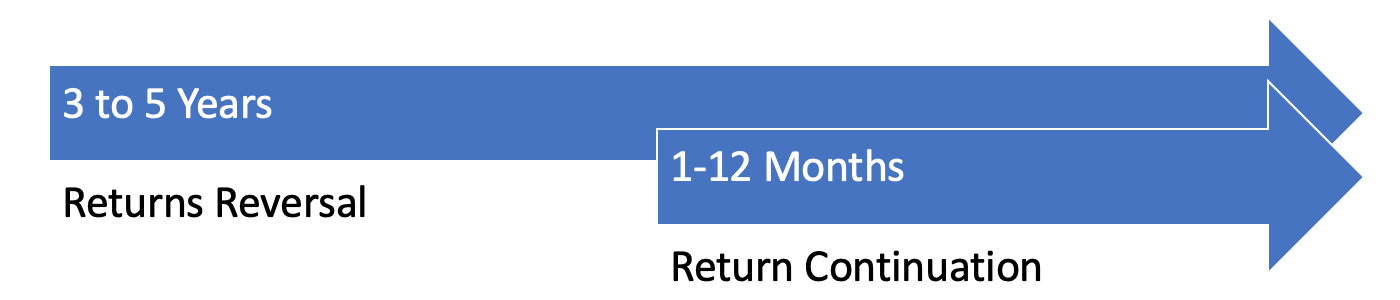
\includegraphics[scale=.4]{sumup.png}
              \end{figure}
        \item On the one hand, returns appear to exhibit continuation, or momentum, in the short to medium run. On the other hand, there is also a tendency toward reversals, or fundamental reversion, in the long run
    \end{itemize}
\end{frame}
%%%%%%%%%%%%%%%%%%%%%%%%%%%%%%%%%%%%%%%%%%%%%%%%%%%%%%%%%%%%%%%%%%%%%%%%%%%%%%%

%%%%%%%%%%%%%%%%%%%%%%%%%%%%%%%%%%%%%%%%%%%%%%%%%%%%%%%%%%%%%%%%%%%%%%%%%%%%%%%
\begin{frame}{Challenge to Theories}
    \begin{itemize}
        \item Patterns in average returns that are not explained by the CAPM are called anomalies.
        \item Fama and French (1996): The authors believe that their three-factor model can account for the overreaction evidence, but not for the continuation of short-term returns (underreaction).
        \item FF (96), state ‍‍‍‍`our model cannot explain the continuation of short-term returns documented by Jegadeesh and Titman (1993). As it does for long-term returns, this pattern in the HML slopes predicts reversal rather than continuation for future returns.`
        \item The evidence presents a challenge to the EMH because it suggests that in a variety of markets, sophisticated investors can earn superior returns by taking advantage of underreaction and overreaction without bearing extra risk.
    \end{itemize}
\end{frame}
%%%%%%%%%%%%%%%%%%%%%%%%%%%%%%%%%%%%%%%%%%%%%%%%%%%%%%%%%%%%%%%%%%%%%%%%%%%%%%%

%%%%%%%%%%%%%%%%%%%%%%%%%%%%%%%%%%%%%%%%%%%%%%%%%%%%%%%%%%%%%%%%%%%%%%%%%%%%%%%
\begin{frame}{Relation to Behavioral Finance}
    \begin{itemize}
        \item This evidence also presents a challenge to behavioral finance theory because early models do not successfully explain the facts.
        \item Some aspects of the patterns seem contradictory, such as apparent market underreaction in some contexts and overreaction in others.
        \item Barberis, Shleifer, Vishny (1998) propose a model based on empirical psychological pieces of evidence to explain this behavior.
              \begin{enumerate}
                  \item Behavioral heuristic known as representativeness.
                  \item Conservatism.
              \end{enumerate}
    \end{itemize}
\end{frame}
%%%%%%%%%%%%%%%%%%%%%%%%%%%%%%%%%%%%%%%%%%%%%%%%%%%%%%%%%%%%%%%%%%%%%%%%%%%%%%%

%%%%%%%%%%%%%%%%%%%%%%%%%%%%%%%%%%%%%%%%%%%%%%%%%%%%%%%%%%%%%%%%%%%%%%%%%%%%%%%
\begin{frame}{Explanation by Behavioral Finance}
    \begin{itemize}
        \item Daniel et al. (98) propose a model based on two well-known psychological biases: investor overconfidence, biased self-attribution.
        \item DeBondt and Thaler (1995) state that `perhaps the most robust finding in the psychology of judgment is that people are overconfident.`
        \item Further, some evidence suggests that experts tend to be more overconfident than relatively inexperienced individuals.
        \item Psychological evidence also indicates that overconfidence is more severe for tasks that require judgment than for mechanical tasks (e.g., solving arithmetic problems); and more severe for tasks with delayed feedback as opposed to tasks that provide immediate and conclusive outcome feedback.
    \end{itemize}
\end{frame}
%%%%%%%%%%%%%%%%%%%%%%%%%%%%%%%%%%%%%%%%%%%%%%%%%%%%%%%%%%%%%%%%%%%%%%%%%%%%%%%

%%%%%%%%%%%%%%%%%%%%%%%%%%%%%%%%%%%%%%%%%%%%%%%%%%%%%%%%%%%%%%%%%%%%%%%%%%%%%%%
\section{Methodology}
%%%%%%%%%%%%%%%%%%%%%%%%%%%%%%%%%%%%%%%%%%%%%%%%%%%%%%%%%%%%%%%%%%%%%%%%%%%%%%%

%%%%%%%%%%%%%%%%%%%%%%%%%%%%%%%%%%%%%%%%%%%%%%%%%%%%%%%%%%%%%%%%%%%%%%%%%%%%%%%
\begin{frame}{Methodology}
    \begin{itemize}
        \item Profitable performance of the relative strength strategies implies that stocks that generate higher than average returns in one period also generate higher than average returns in the period that follows and vise versa.
              \[
                  \mathrm{E}\left(r_{i t}-\bar{r}_{t} \mid r_{i t-1}-\bar{r}_{t-1}  \gtrless  0\right)\gtrless 0
              \]
        \item If we assume a simple one-factor model.
              \[
                  \begin{array}{rlr}
                      r_{i t}                                           & =\mu_{i}+b_{i} f_{t}+e_{i t},                    \\
                      \mathrm{E}\left(f_{t}\right)                      & =0                            &                  \\
                      \mathrm{E}\left(e_{i t}\right)                    & =0                            &                  \\
                      \operatorname{Cov}\left(e_{i t}, f_{t}\right)     & =0,                           & \forall i        \\
                      \operatorname{Cov}\left(e_{i t}, e_{j t-1}\right) & =0,                           & \forall i \neq j
                  \end{array}
              \]
    \end{itemize}
\end{frame}
%%%%%%%%%%%%%%%%%%%%%%%%%%%%%%%%%%%%%%%%%%%%%%%%%%%%%%%%%%%%%%%%%%%%%%%%%%%%%%%

%%%%%%%%%%%%%%%%%%%%%%%%%%%%%%%%%%%%%%%%%%%%%%%%%%%%%%%%%%%%%%%%%%%%%%%%%%%%%%%
\begin{frame}{Decompostion}
    \begin{itemize}
        \item In other words:
              \[
                  \mathrm{Cov}\left\{\left(r_{i t}-\bar{r}_{t}\rigth) \left(r_{i t-1}-\bar{r}_{t-1}\right) \right\} > 0
              \]
        \item Profits given in the above expression can be decomposed into the following three terms:
              \[
                  \mathrm{E}\left\{ \left(r_{i t}-\overline{r}_{t}\right)\left(r_{i t-1}-\overline{r}_{t-1}\right) \right\}= \sigma_{\mu}^{2}+\sigma_{b}^{2} \operatorname{Cov}\left(f_{t}, f_{t-1}\right)
                  +\overline{\operatorname{Cov}}_{i}\left(e_{i t}, e_{i t-1}   \right)
              \]
        \item where \(\sigma_{\mu}^{2}\) and \(\sigma_{b}^{2}\) are the cross-sectional variances of expected returns and factor sensitivities respectively.
    \end{itemize}
\end{frame}
%%%%%%%%%%%%%%%%%%%%%%%%%%%%%%%%%%%%%%%%%%%%%%%%%%%%%%%%%%%%%%%%%%%%%%%%%%%%%%%

%%%%%%%%%%%%%%%%%%%%%%%%%%%%%%%%%%%%%%%%%%%%%%%%%%%%%%%%%%%%%%%%%%%%%%%%%%%%%%%
\begin{frame}{Sources of the Relative Strength Profits}
    \begin{itemize}
        \item This \(\sigma_{\mu}^{2}+\sigma_{b}^{2} \operatorname{Cov}\left(f_{t}, f_{t-1}\right)
              +\overline{\operatorname{Cov}}_{i}\left(e_{i t}, e_{i t-1}\right) \)
              suggests three potential sources.
        \item Since realized returns contain a component related to expected returns, securities that experience relatively high returns in one period can be expected to have higher than average returns in the following period.
        \item The second term is related to the potential to time the factor. If the factor portfolio returns exhibit positive serial correlation, the relative strength strategy will tend to pick stocks with high b'self when the conditional expectation of the factor portfolio return is high.
        \item The last term in the above expression is the average serial covariance of the idiosyncratic components of security returns.

    \end{itemize}
\end{frame}
%%%%%%%%%%%%%%%%%%%%%%%%%%%%%%%%%%%%%%%%%%%%%%%%%%%%%%%%%%%%%%%%%%%%%%%%%%%%%%%

%%%%%%%%%%%%%%%%%%%%%%%%%%%%%%%%%%%%%%%%%%%%%%%%%%%%%%%%%%%%%%%%%%%%%%%%%%%%%%%
\begin{frame}{Decompostion Implications}
    \begin{itemize}
        \item To assess whether the existence of relative strength profits imply market inefficiency, it is important to identify the sources of the profits.
        \item If the profits are due to either the first or the second term in the last expression they may be attributed to compensation for bearing systematic risk and need not be an indication of market inefficiency.
        \item However, if the superior performance of the relative strength strategies is due to the third term, then the results would suggest market inefficiency.
        \item JT(93) find that profitability of these strategies are not due to their systematic risk or to delayed stock price reactions to common factors.
    \end{itemize}
\end{frame}
%%%%%%%%%%%%%%%%%%%%%%%%%%%%%%%%%%%%%%%%%%%%%%%%%%%%%%%%%%%%%%%%%%%%%%%%%%%%%%%

%%%%%%%%%%%%%%%%%%%%%%%%%%%%%%%%%%%%%%%%%%%%%%%%%%%%%%%%%%%%%%%%%%%%%%%%%%%%%%%
\begin{frame}{Trading Strategies}
    \begin{itemize}
        \item The strategies we consider select stocks based on their returns over the past 1, 2, 3, or 4 quarters. We also consider holding periods that vary from 1 to 4 quarters. This gives a total of 16 strategies.
              \begin{figure}
                  \centering
                  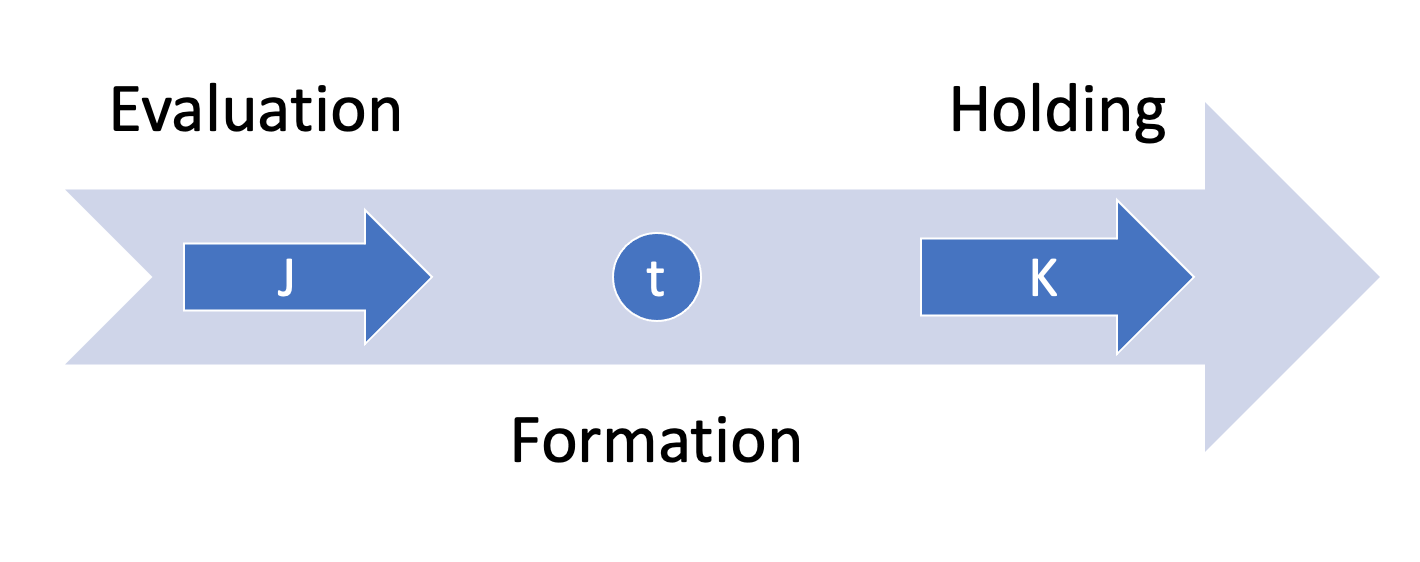
\includegraphics[scale=.4]{strategies.png}
              \end{figure}
    \end{itemize}
\end{frame}
%%%%%%%%%%%%%%%%%%%%%%%%%%%%%%%%%%%%%%%%%%%%%%%%%%%%%%%%%%%%%%%%%%%%%%%%%%%%%%%

%%%%%%%%%%%%%%%%%%%%%%%%%%%%%%%%%%%%%%%%%%%%%%%%%%%%%%%%%%%%%%%%%%%%%%%%%%%%%%%
\section{Preliminary Results}
%%%%%%%%%%%%%%%%%%%%%%%%%%%%%%%%%%%%%%%%%%%%%%%%%%%%%%%%%%%%%%%%%%%%%%%%%%%%%%%

%%%%%%%%%%%%%%%%%%%%%%%%%%%%%%%%%%%%%%%%%%%%%%%%%%%%%%%%%%%%%%%%%%%%%%%%%%%%%%%
\begin{frame}{Data}
    \begin{itemize}
        \item Date Span: 1380/01 to 1399/09.
        \item We use adjusted Prices.
              \begin{center}
                  \begin{tabular}{l r r}
                                             & Monthly     & Annually   \\ \cline{2-3}
                      Number                 & 236         & 20         \\
                      Positive Return Number & 164         & 17         \\
                      Negative Return Number & 71          & 3          \\ \hline
                      EWI Returns            &             &            \\ \hline
                      Mean                   & 3.43\%      & 57.73\%    \\
                      Var.                   & 0.0050      & 0.6598     \\
                      STD                    & 0.0711      & 0.8123     \\
                      Median                 & 1.98\%      & 31.06\%    \\
                      Max.                   & 43.23\%     & 369.51\%   \\
                      Min.                   & -11.20\%    & -8.69\%    \\
                      Cumulative             & 172687.60\% & 76764.42\%
                  \end{tabular}
              \end{center}
    \end{itemize}
\end{frame}
%%%%%%%%%%%%%%%%%%%%%%%%%%%%%%%%%%%%%%%%%%%%%%%%%%%%%%%%%%%%%%%%%%%%%%%%%%%%%%%

%%%%%%%%%%%%%%%%%%%%%%%%%%%%%%%%%%%%%%%%%%%%%%%%%%%%%%%%%%%%%%%%%%%%%%%%%%%%%%%
\begin{frame}{Backtest Results, Panel A}{Without 7 Days Formation Lag}
    \begin{table}
        \tiny
        \centering
        \begin{tabular}{llrSSSScSSSS}
               & J        & K= & \multicolumn{1}{c}{3} & \multicolumn{1}{c}{6} & \multicolumn{1}{c}{9} & \multicolumn{1}{c}{12} \\
            \midrule
            3  & Sell     &    & -0.0290               & -0.0241               & -0.0303               & -0.0278                \\
               &          &    & (5.89)                & (5.84)                & (2.98)                & (3.24)                 \\
            3  & Buy      &    & 0.0297                & 0.0278                & 0.0263                & 0.0245                 \\
               &          &    & (5.93)                & (6.13)                & (6.33)                & (6.28)                 \\
            3  & Buy-sell &    & 0.0587                & 0.0519                & 0.0566                & 0.0523                 \\
               &          &    & (6.36)                & (6.26)                & (4.49)                & (4.74)                 \\
            6  & Sell     &    & -0.0455               & -0.0385               & -0.0331               & -0.0316                \\
               &          &    & (2.16)                & (2.48)                & (2.74)                & (3.05)                 \\
            6  & Buy      &    & 0.0324                & 0.0306                & 0.0291                & 0.0266                 \\
               &          &    & (6.23)                & (6.31)                & (6.25)                & (6.02)                 \\
            6  & Buy-sell &    & 0.0779                & 0.0691                & 0.0621                & 0.0582                 \\
               &          &    & (3.37)                & (3.87)                & (4.26)                & (4.51)                 \\
            9  & Sell     &    & -0.0259               & -0.0251               & -0.0401               & -0.0372                \\
               &          &    & (5.19)                & (5.32)                & (2.57)                & (2.86)                 \\
            9  & Buy      &    & 0.0313                & 0.0305                & 0.0279                & 0.0257                 \\
               &          &    & (5.83)                & (6.09)                & (5.78)                & (5.62)                 \\
            9  & Buy-sell &    & 0.0572                & 0.0555                & 0.0680                & 0.0629                 \\
               &          &    & (6.18)                & (6.14)                & (3.81)                & (4.09)                 \\
            12 & Sell     &    & -0.0249               & -0.0250               & -0.0283               & -0.0290                \\
               &          &    & (5.21)                & (5.19)                & (5.73)                & (6.00)                 \\
            12 & Buy      &    & 0.0296                & 0.0292                & 0.0272                & 0.0253                 \\
               &          &    & (5.56)                & (5.50)                & (5.31)                & (5.21)                 \\
            12 & Buy-sell &    & 0.0545                & 0.0541                & 0.0555                & 0.0543                 \\
               &          &    & (5.97)                & (5.74)                & (5.85)                & (5.89)                 \\
            \bottomrule
        \end{tabular}
    \end{table}
\end{frame}
%%%%%%%%%%%%%%%%%%%%%%%%%%%%%%%%%%%%%%%%%%%%%%%%%%%%%%%%%%%%%%%%%%%%%%%%%%%%%%%

%%%%%%%%%%%%%%%%%%%%%%%%%%%%%%%%%%%%%%%%%%%%%%%%%%%%%%%%%%%%%%%%%%%%%%%%%%%%%%%
\begin{frame}{Backtest Results, Panel B}{With 7 Days Formation Lag}
    \begin{table}
        \tiny
        \centering
        \begin{tabular}{llrSSSScSSSS}
               & J        & K= & \multicolumn{1}{c}{3} & \multicolumn{1}{c}{6} & \multicolumn{1}{c}{9} & \multicolumn{1}{c}{12} \\
            \midrule
            3  & Sell     &    & -0.0298               & -0.0242               & -0.0303               & -0.0278                \\
               &          &    & (5.67)                & (5.39)                & (3.01)                & (3.24)                 \\
            3  & Buy      &    & 0.0300                & 0.0277                & 0.0261                & 0.0244                 \\
               &          &    & (5.50)                & (5.65)                & (5.87)                & (5.80)                 \\
            3  & Buy-sell &    & 0.0598                & 0.0518                & 0.0564                & 0.0522                 \\
               &          &    & (5.91)                & (5.73)                & (4.39)                & (4.60)                 \\
            6  & Sell     &    & -0.0460               & -0.0385               & -0.0340               & -0.0327                \\
               &          &    & (2.20)                & (2.50)                & (2.81)                & (3.14)                 \\
            6  & Buy      &    & 0.0311                & 0.0307                & 0.0293                & 0.0268                 \\
               &          &    & (5.69)                & (6.08)                & (6.07)                & (5.69)                 \\
            6  & Buy-sell &    & 0.0771                & 0.0692                & 0.0634                & 0.0595                 \\
               &          &    & (3.32)                & (3.85)                & (4.26)                & (4.49)                 \\
            9  & Sell     &    & -0.0253               & -0.0259               & -0.0404               & -0.0387                \\
               &          &    & (4.63)                & (5.06)                & (2.65)                & (2.99)                 \\
            9  & Buy      &    & 0.0308                & 0.0303                & 0.0277                & 0.0258                 \\
               &          &    & (5.60)                & (5.76)                & (5.38)                & (5.23)                 \\
            9  & Buy-sell &    & 0.0561                & 0.0562                & 0.0681                & 0.0645                 \\
               &          &    & (5.62)                & (5.73)                & (3.81)                & (4.12)                 \\
            12 & Sell     &    & -0.0269               & -0.0273               & -0.0284               & -0.0299                \\
               &          &    & (4.79)                & (5.00)                & (5.31)                & (5.54)                 \\
            12 & Buy      &    & 0.0292                & 0.0282                & 0.0274                & 0.0257                 \\
               &          &    & (5.30)                & (5.11)                & (5.00)                & (4.95)                 \\
            12 & Buy-sell &    & 0.0560                & 0.0556                & 0.0558                & 0.0556                 \\
               &          &    & (5.50)                & (5.40)                & (5.43)                & (5.52)                 \\
            \bottomrule
        \end{tabular}
    \end{table}
\end{frame}
%%%%%%%%%%%%%%%%%%%%%%%%%%%%%%%%%%%%%%%%%%%%%%%%%%%%%%%%%%%%%%%%%%%%%%%%%%%%%%%

%%%%%%%%%%%%%%%%%%%%%%%%%%%%%%%%%%%%%%%%%%%%%%%%%%%%%%%%%%%%%%%%%%%%%%%%%%%%%%%
\begin{frame}{Remarks About Our Results}
    \begin{itemize}
        \item All results are statistically significant at 1\% level.
        \item In the opposite of momentum literature, all short strategies yield negative returns.
        \item There are two main questions, are these profits due to investor sentiments, put differently do we have market under- over-reaction?
        \item Comparing to counter part US results sell strategies are more profitable.
    \end{itemize}
\end{frame}
%%%%%%%%%%%%%%%%%%%%%%%%%%%%%%%%%%%%%%%%%%%%%%%%%%%%%%%%%%%%%%%%%%%%%%%%%%%%%%%

%%%%%%%%%%%%%%%%%%%%%%%%%%%%%%%%%%%%%%%%%%%%%%%%%%%%%%%%%%%%%%%%%%%%%%%%%%%%%%%
\begin{frame}{Remarks About Our Results}
    \begin{itemize}
        \item For US, the most successful zero-cost strategy selects stocks based on their returns over the previous 12 months and then holds the portfolio for 3 months.
        \item For TSE, the most successful strategy selects stocks based on their returns over the previous 6 months and then holds the portfolio for 3 months. But it is not the same strategy as the US.
    \end{itemize}
\end{frame}
%%%%%%%%%%%%%%%%%%%%%%%%%%%%%%%%%%%%%%%%%%%%%%%%%%%%%%%%%%%%%%%%%%%%%%%%%%%%%%%

%%%%%%%%%%%%%%%%%%%%%%%%%%%%%%%%%%%%%%%%%%%%%%%%%%%%%%%%%%%%%%%%%%%%%%%%%%%%%%%
\begin{frame}{Possible Explanations}
    \begin{itemize}
        \item For long strategies, by additional shreds of evidence maybe we can attribute profits to under- over-reaction.
        \item For negative short strategies, results could be due to share support by institutional investors.
        \item Combining this result with institutional/individual transaction data may support the share support hypothesis.
        \item These are hypothetical returns. In fact, in practice, we do not have short trading.
        \item In a Counterfactual manner, if we had short trading, there might be positive returns to short strategies and lower positive returns to buy strategies.
    \end{itemize}
\end{frame}
%%%%%%%%%%%%%%%%%%%%%%%%%%%%%%%%%%%%%%%%%%%%%%%%%%%%%%%%%%%%%%%%%%%%%%%%%%%%%%%

%%%%%%%%%%%%%%%%%%%%%%%%%%%%%%%%%%%%%%%%%%%%%%%%%%%%%%%%%%%%%%%%%%%%%%%%%%%%%%%
\begin{frame}{In What Follows}
    \begin{itemize}
        \item Decomposing of profits to different sources.
        \item Exploring further why sell strategies are not profitable.
        \item (Is there any relation to allowed daily price variation?)
    \end{itemize}
\end{frame}
%%%%%%%%%%%%%%%%%%%%%%%%%%%%%%%%%%%%%%%%%%%%%%%%%%%%%%%%%%%%%%%%%%%%%%%%%%%%%%%

%%%%%%%%%%%%%%%%%%%%%%%%%%%%%%%%%%%%%%%%%%%%%%%%%%%%%%%%%%%%%%%%%%%%%%%%%%%%%%%
\begin{frame}
    \begin{center}
        \huge
        THANKS.
    \end{center}
\end{frame}
%%%%%%%%%%%%%%%%%%%%%%%%%%%%%%%%%%%%%%%%%%%%%%%%%%%%%%%%%%%%%%%%%%%%%%%%%%%%%%%



%%%%%%%%%%%%%%%%%%%%%%%%%%%%%%% Document End %%%%%%%%%%%%%%%%%%%%%%%%%%%%%%%%%%
\end{document}
%%%%%%%%%%%%%%%%%%%%%%%%%%%%%%%%%%%%%%%%%%%%%%%%%%%%%%%%%%%%%%%%%%%%%%%%%%%%%%%
